\mode*
\section[Def. Problema]{Definici\'on del problema}
\label{sec:problema}

\mode<presentation>{
  \begin{frame}
    \transduration{1}
    \frametitle{Cu\'al es el problema?}
    \framesubtitle{Generaci\'on de rob\'otica b\'ipeda y soluci\'on a sus problemas}
    \begin{center}
      \LARGE \textbf{\textcolor{blueun}{Definici\'on del problema}}
    \end{center}      
  \end{frame}
}
\subsection[Identificaci\'on]{Identificaci\'on}
\mode<presentation>{
  \begin{frame}
    \transduration<1->{1}
    \frametitle{Qu\'e pas\'o?}
    \framesubtitle{Causas del receso en al investigaci\'on}
    \begin{center}
      \only<1>{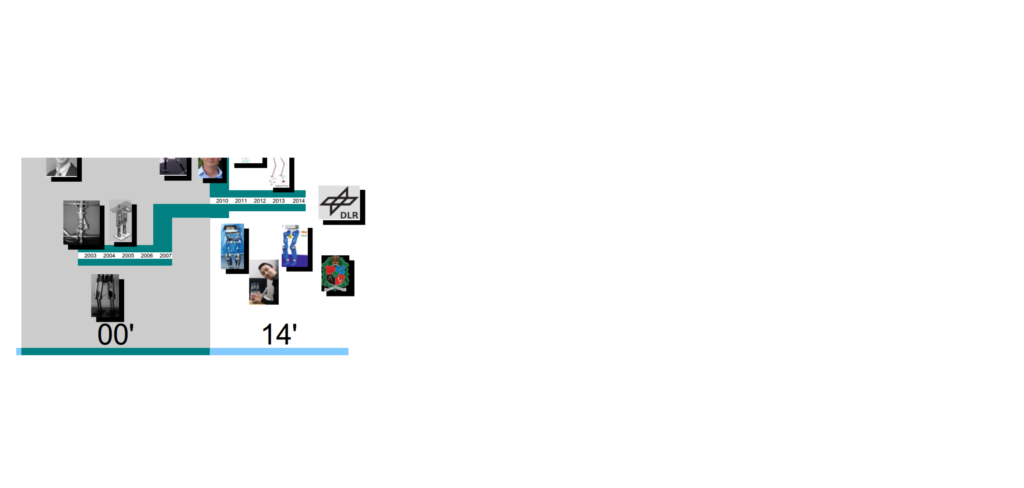
\includegraphics[width=10.5cm]{../images/Problema_0.png}}
      \only<2>{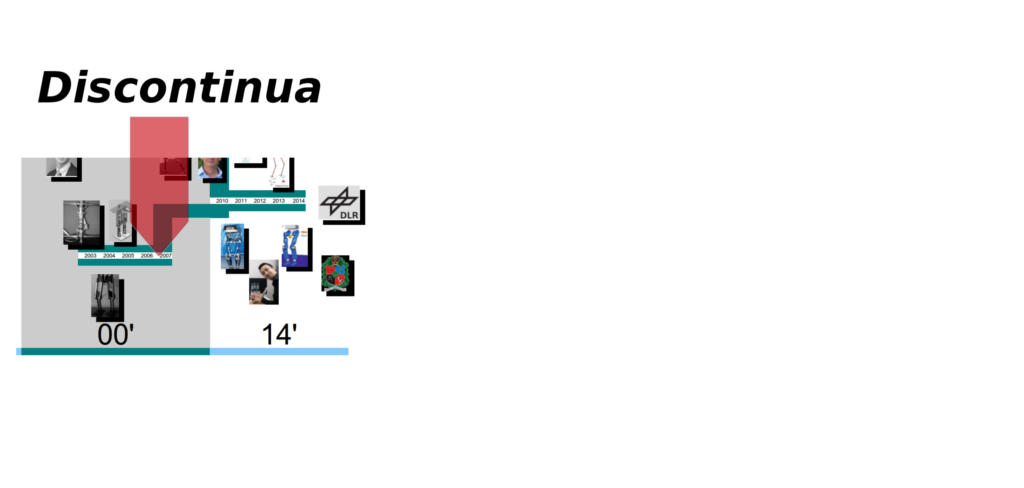
\includegraphics[width=10.5cm]{../images/Problema_1.png}}
    \end{center}      
  \end{frame}
}
Se observa un estancamiento en la aplicaci\'on de los conocimientos de la Universidad en el \'area de la rob\'otica b\'ipeda que sean integrados de forma funcional en este campo. Diferentes materias de pregrado y posgrado que reflejan dicho conocimiento como: Rob\'otica, Din\'amica de robots, Biom\'ecanica, T\'ecnicas de control, Identificaci\'on de sistemas, Optimizaci\'on, Control de robots, Control Robusto, Sistemas embebidos, Computaci\'on flexible, Computaci\'on gr\'afica y varias m\'as, deben ser integradas para abordar la soluci\'on de diversos problemas presentes en la caminata rob\'otica, como se reporta en todas las referencias citadas de este documento.\par
Una de las posibles causas por las que se haya detenido el avance de este campo es tal vez que el conocimiento requerido para ser integraci\'on proviene de distintas disciplinas.\par

\subsection[Formulaci\'on]{Formulaci\'on del problema}
\mode<presentation>{
  \begin{frame}
    \transduration<1->{1}
    \frametitle{Qu\'e se quiere resolver?}
    \framesubtitle{Regreso a la frontera}
    \begin{center}
      \only<1>{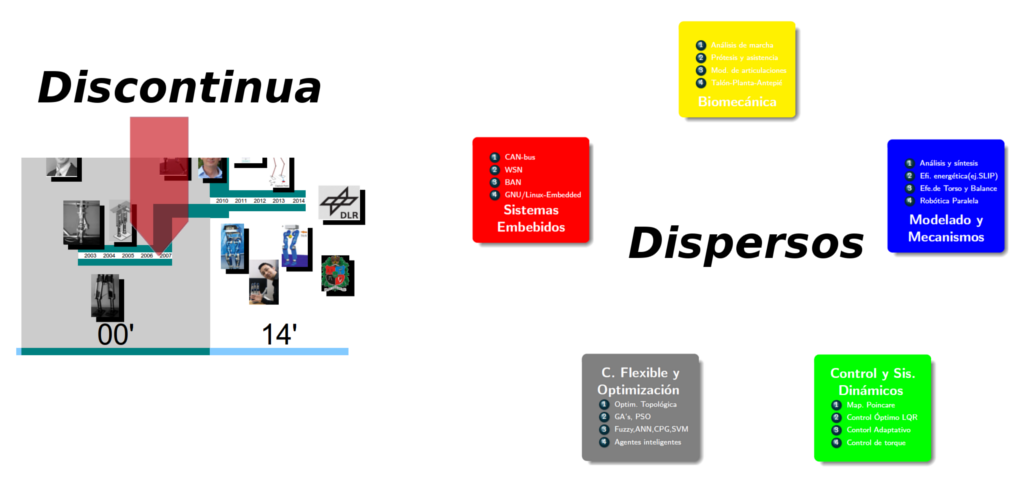
\includegraphics[width=10.5cm]{../images/Problema_2.png}}
      \only<2>{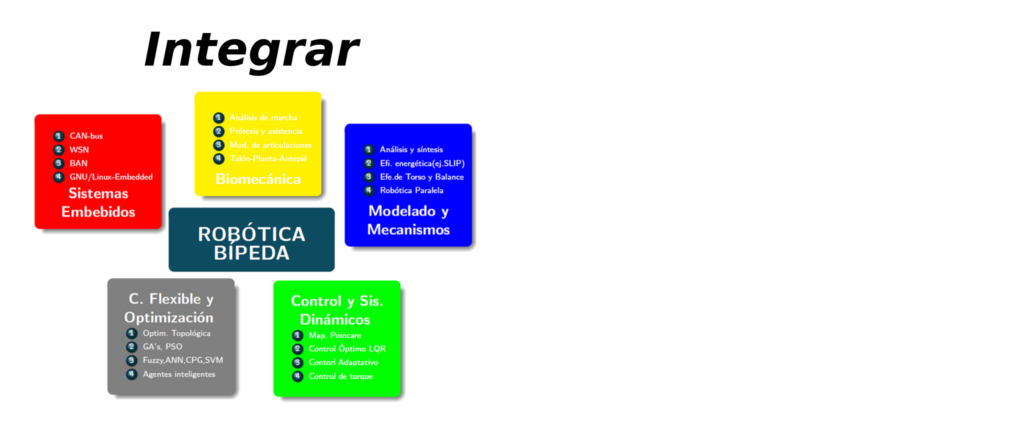
\includegraphics[width=10.5cm]{../images/Problema_3.png}}
    \end{center}      
  \end{frame}
}
El problema central a trabajar es: poder proponer, analizar e implementar en una plataforma b\'ipeda real y/o simulada, estrategias de control de caminata, control de direcci\'on, balance ante perturbaciones, generaci\'on y planeaci\'on de trayectorias, control de trote, control de saltos, implementaci\'on de agentes inteligentes, as\'i como dise\~nos que sean eficientes en el consumo de energ\'ia y que funcionen con los actuadores disponibles. Todos los problemas mencionados son de inter\'es mundial en cientos de laboratorio en el planeta.

